\chapter{Introduction}
\section{Project Background}

The Colebrooke Subdivision is a proposed residential development located in the City of Florence, Rankin County, Mississippi, approximately 1{,}825~ft west of Seventh Day Road on the north side of Lewis Street~\cite{ProjectD_Colebrooke_2020}. The site consists of previously undeveloped land characterized by gently rolling terrain and surrounding residential and semi-urban land uses. The development is part of ongoing regional growth and is intended to expand residential capacity while providing essential infrastructure to support future occupants.

The project involves the preparation of a comprehensive civil engineering design to establish the infrastructure required for a functional residential community. These infrastructure components include roadway systems, stormwater management facilities, and a sanitary sewer network designed to safely collect and convey wastewater generated by the subdivision to the existing municipal sewer system. The preliminary subdivision layout defines internal road alignments, lot configurations, and utility corridors in accordance with municipal planning requirements and design standards~\cite{ProjectD_Colebrooke_2020}.

\begin{figure}[H]
    \centering
    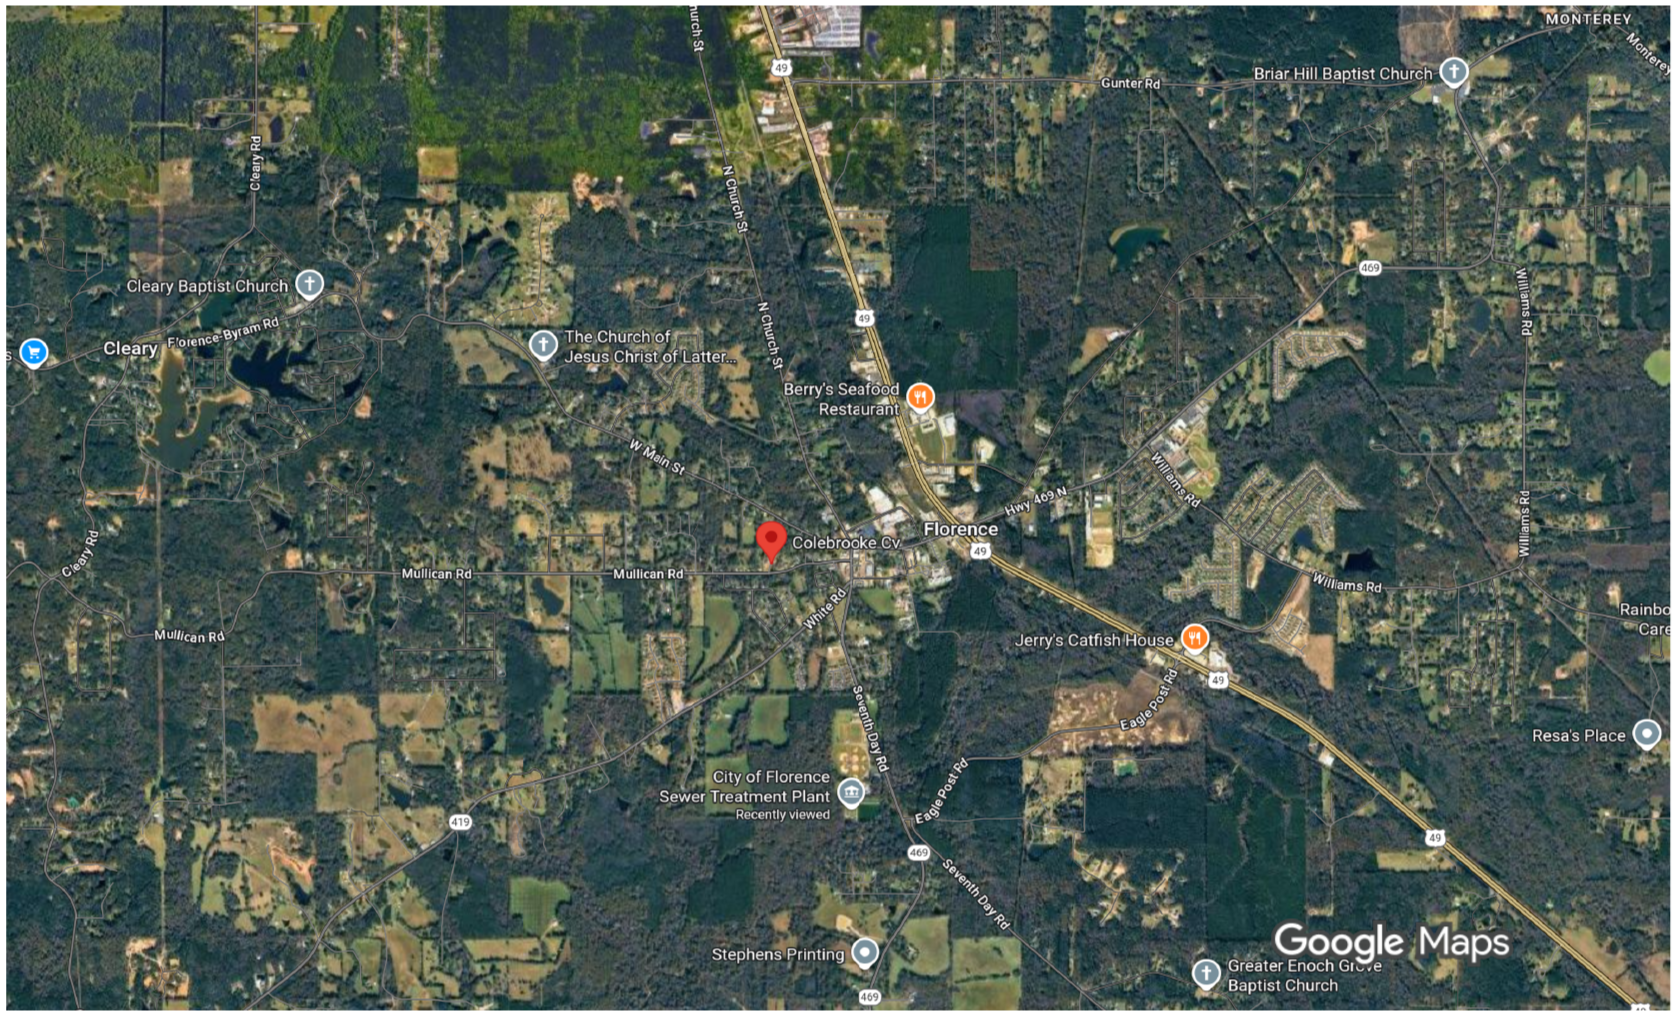
\includegraphics[width=0.76\textwidth]{figures/site.png}
    \caption{Colebrooke Subdivision Location Map.}
    \label{fig:colebrooke_location}
\end{figure}

The infrastructure systems within the subdivision are designed to operate as an integrated network that supports long-term functionality, environmental protection, and public health. Within this network, the sanitary sewer system plays a critical role by ensuring the reliable collection and transport of domestic wastewater. The performance of this system is essential for maintaining safe living conditions and preventing environmental contamination, making it a key component of the overall subdivision design.


\section{Need for a Pump Station}

The sanitary sewer system proposed for the Colebrooke Subdivision is designed to collect wastewater from individual residential lots through a gravity-driven network and convey it to the existing municipal sewer system. Under ideal conditions, gravity flow provides a reliable and energy-efficient means of wastewater transport. However, the topographic characteristics of the project site impose a fundamental limitation on the use of a gravity-only system.

The gently rolling terrain of the subdivision results in a local low point within the development where wastewater accumulates. The elevation of this low point is insufficient to allow continuous gravity discharge to the downstream municipal sewer connection. As a result, wastewater cannot be conveyed entirely by gravity without risking surcharge conditions, reduced hydraulic performance, or system failure.

To overcome this elevation constraint, a pump station and pressure force main are required to lift wastewater from the subdivision’s low point and convey it to the downstream municipal sewer system. The pump station provides the hydraulic energy necessary to overcome both the static elevation difference and the frictional losses within the force main, thereby ensuring continuous and controlled wastewater transport.

The pump station and force main therefore serve as a critical interface between the internal gravity sewer network and the external municipal system. The reliability of this subsystem is essential for maintaining uninterrupted wastewater conveyance, preventing system backups, and protecting public health and the surrounding environment. Consequently, the design must ensure adequate hydraulic capacity, operational redundancy, and compliance with applicable wastewater design standards, including the \textit{Guidance for the Design of Publicly Owned Wastewater Facilities} issued by the Mississippi Department of Environmental Quality (MDEQ) and the \textit{Recommended Standards for Wastewater Facilities} (Ten States Standards)~\cite{MDEQ_DesignGuidance_2025,TenStates_RecommendedStandards_2014}.

Figures~\ref{fig:colebrooke_aerial} and \ref{fig:colebrooke_plat} illustrate the project area and subdivision layout, highlighting the spatial configuration that necessitates the use of a pumping system.

\begin{figure}[H]
    \centering
    \includegraphics[page=2,angle=270,width=\textwidth]{./As-Bulids (1).pdf}
    \caption{Aerial View of the Project Area.}
    \label{fig:colebrooke_aerial}
\end{figure}

\begin{figure}[H]
    \centering
    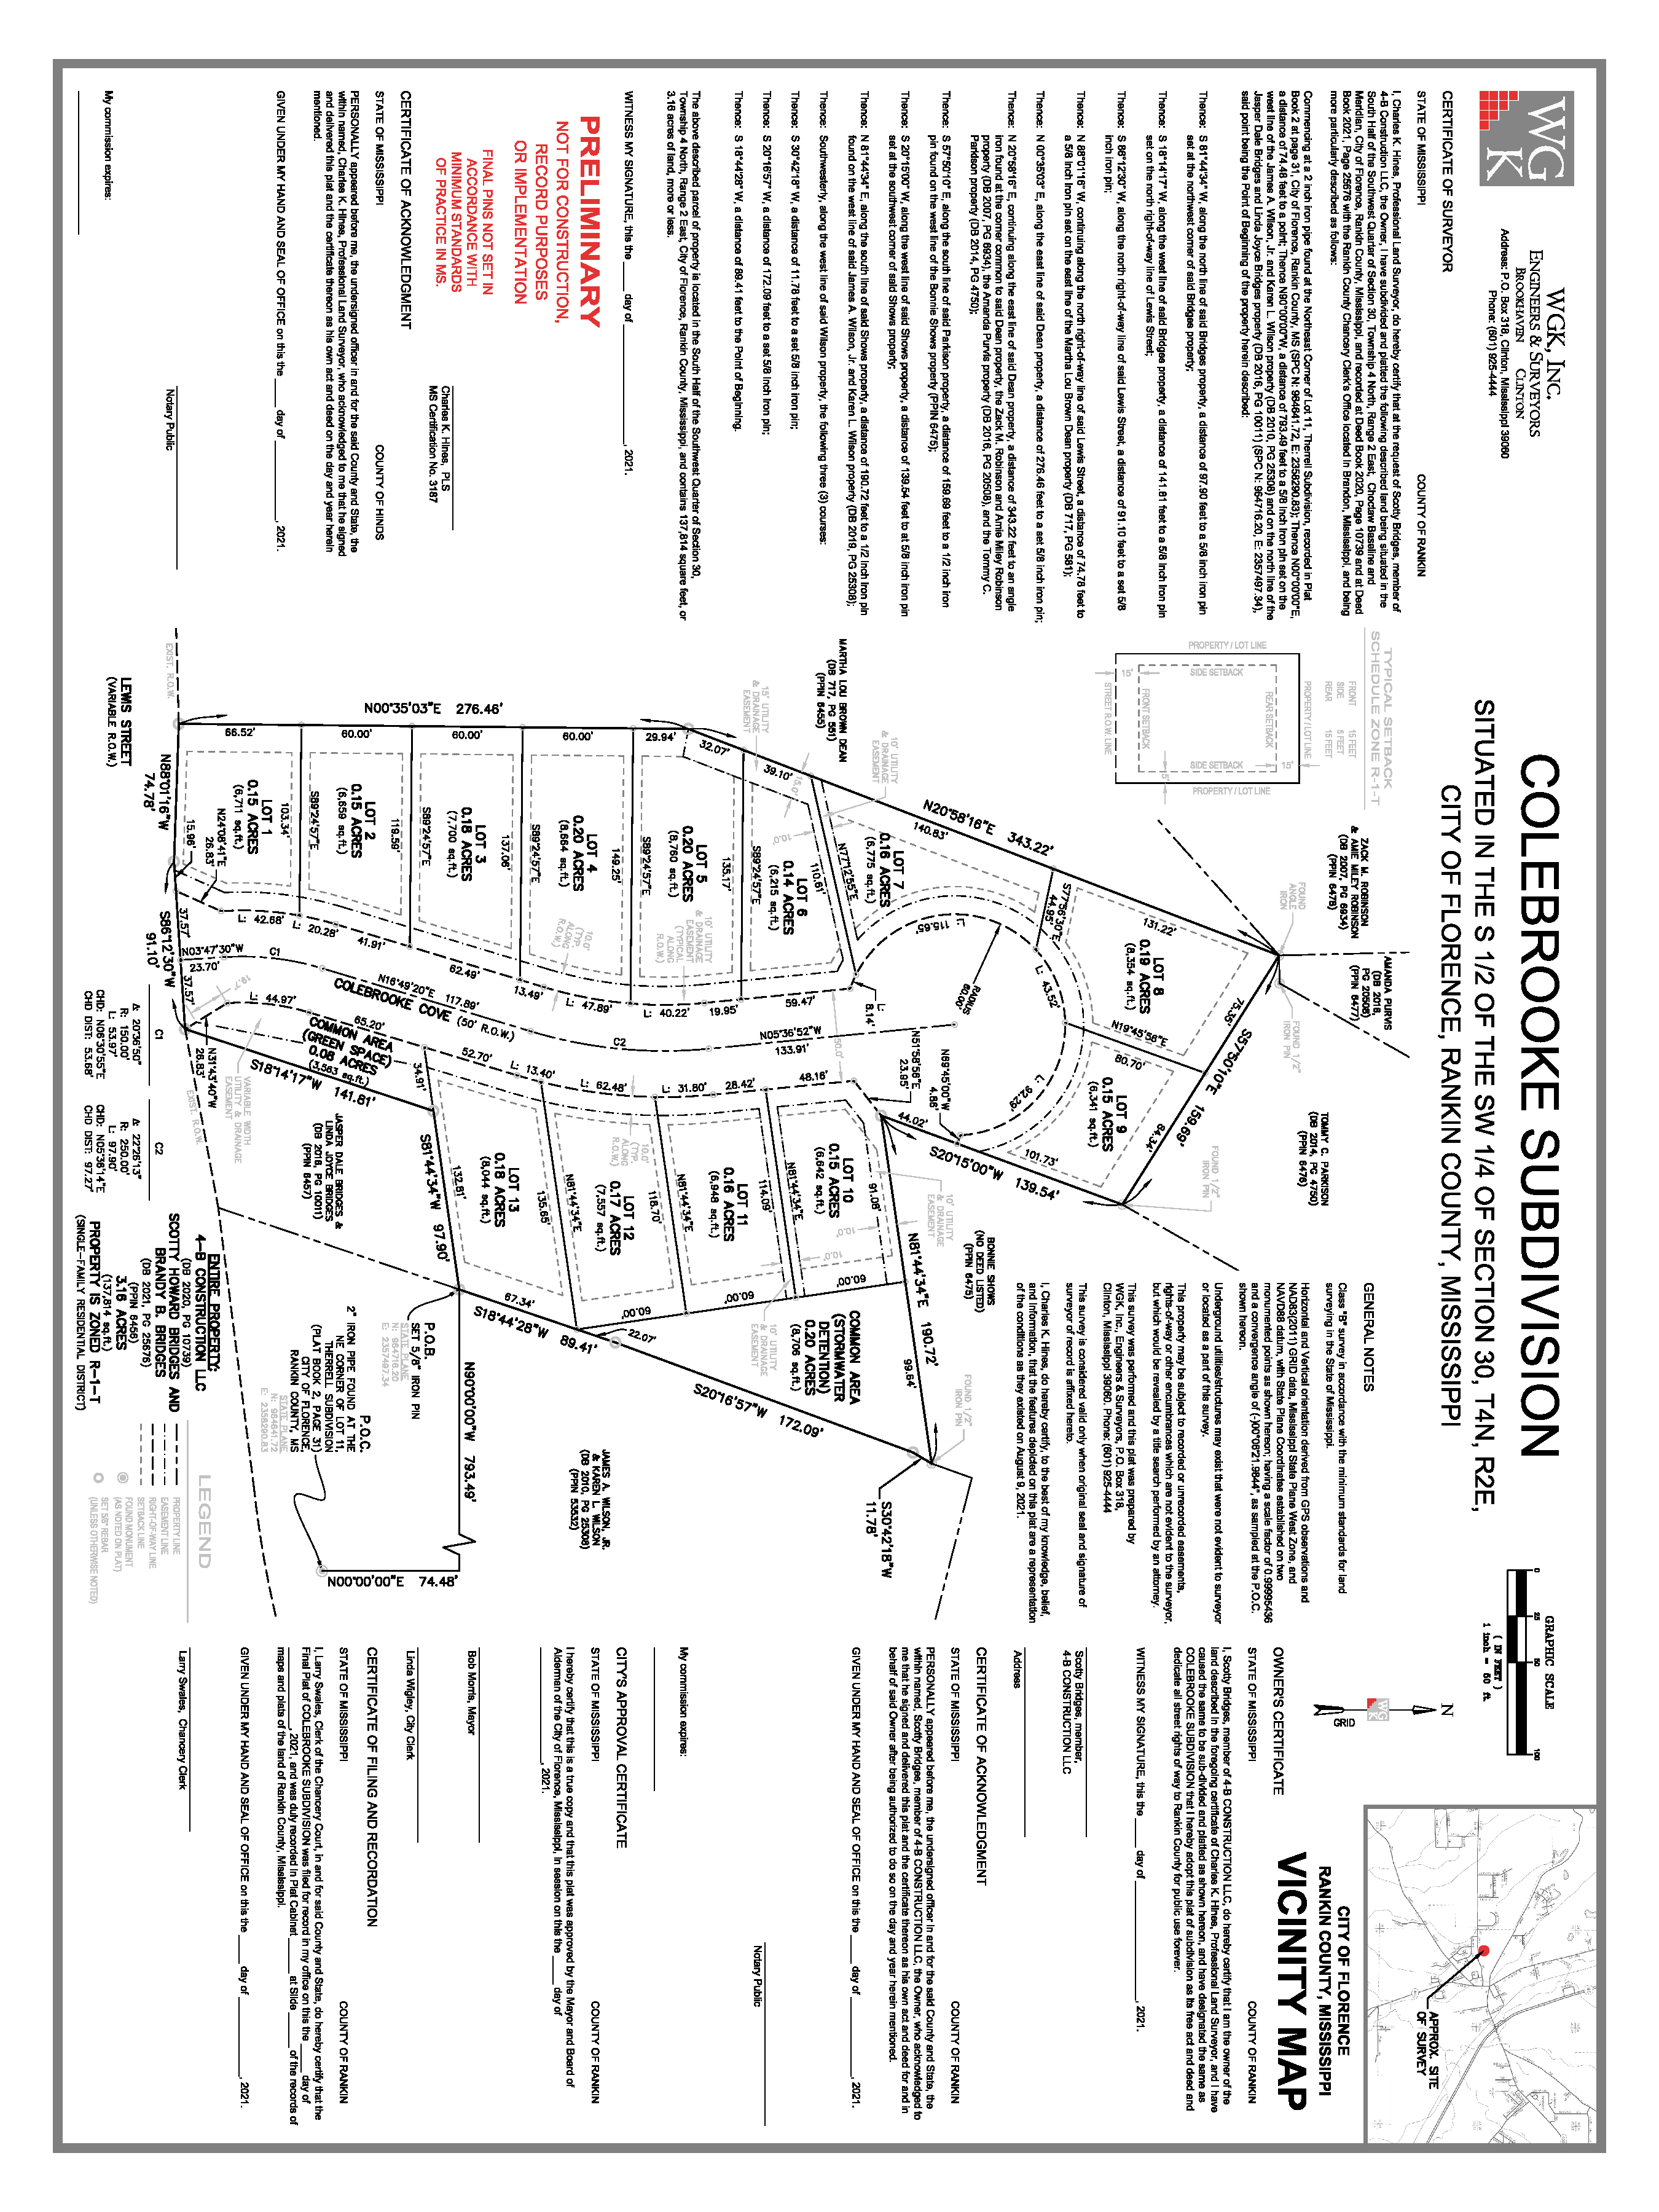
\includegraphics[angle=90,width=\textwidth]{./subdivision_plat_Prelim Plat_Colebrooke Subdivsion (1) (1).pdf}
    \caption{Preliminary Plat of the Colebrooke Subdivision.}
    \label{fig:colebrooke_plat}
\end{figure}



\section{Individual Design Scope and Objectives}

As the author of this report, I, Shams E. Shifat, was responsible for the design and evaluation of the pump station and force main subsystem within the Colebrooke Subdivision sanitary sewer network. This subsystem serves as the critical link between the subdivision’s internal gravity sewer system and the existing municipal sewer network.

My work focused on developing a design that satisfies the hydraulic, operational, and regulatory requirements of the system while accounting for site-specific constraints. The primary tasks included hydraulic analysis of the wastewater conveyance system, sizing and alignment of the force main, and selection of an appropriate pump configuration capable of meeting the system demand.

The design objectives were to ensure reliable wastewater conveyance under peak flow conditions, maintain self-cleansing velocities of at least 2~ft/s within the force main, and provide operational redundancy through a duplex pump configuration. Additional objectives included minimizing headloss within the system, optimizing energy efficiency, and selecting durable, corrosion-resistant materials suitable for long-term service.

The design was developed in accordance with the \textit{Guidance for the Design of Publicly Owned Wastewater Facilities} issued by the Mississippi Department of Environmental Quality (MDEQ) and the \textit{Recommended Standards for Wastewater Facilities} (Ten States Standards)~\cite{MDEQ_DesignGuidance_2025,TenStates_RecommendedStandards_2014}. The resulting design provides a practical and efficient solution for wastewater conveyance within the proposed residential development.


\section{Design Constraints and Assumptions}

The design of the pump station and force main system is governed by a combination of physical site conditions, regulatory requirements, and operational considerations. These constraints define the boundaries within which the hydraulic and structural design must be developed.

A primary physical constraint is the limited elevation difference between the subdivision and the downstream municipal sewer connection, which makes gravity-only wastewater conveyance infeasible. This condition necessitates the inclusion of a pump station to provide the hydraulic head required for wastewater transport. In addition, the site is underlain by moisture-sensitive silty clay soils, which require careful consideration for excavation stability, pipe bedding, and structural support of underground components.

Regulatory constraints are imposed by applicable wastewater design standards, including the \textit{Guidance for the Design of Publicly Owned Wastewater Facilities} issued by the Mississippi Department of Environmental Quality (MDEQ) and the \textit{Recommended Standards for Wastewater Facilities} (Ten States Standards)~\cite{MDEQ_DesignGuidance_2025,TenStates_RecommendedStandards_2014}. These standards establish requirements for system reliability, minimum flow velocity, pump redundancy, and wet well operation.

Operational considerations also influence the design. The system is intended to function under typical residential loading conditions and must ensure continuous and reliable wastewater conveyance. A duplex pump configuration is assumed to provide redundancy, allowing alternating operation and maintaining service during maintenance or equipment failure. The force main is designed to maintain self-cleansing velocities to prevent solids deposition and ensure long-term operational efficiency.

These constraints and assumptions provide the framework for the hydraulic analysis and design decisions presented in the subsequent chapters.
